
%(BEGIN_QUESTION)
% Copyright 2007, Tony R. Kuphaldt, released under the Creative Commons Attribution License (v 1.0)
% This means you may do almost anything with this work of mine, so long as you give me proper credit

Examine this process trend, showing the response of the process variable to a 10\% up-and-down step change in the controller output (placed in manual mode):

$$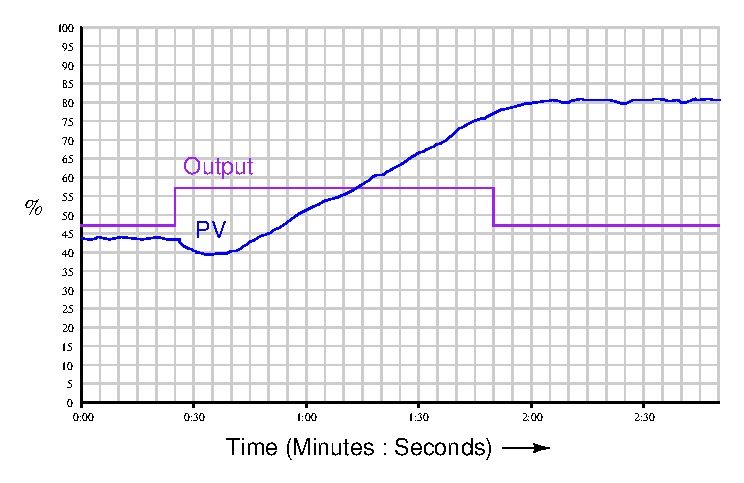
\includegraphics[width=15.5cm]{i01725x01.eps}$$

What characteristics of the process (and its related instrumentation) can you discern from this trend?  Based on this information, hypothesize how you think the controller should be tuned to respond.  In other words, how aggressive should the controller's P, I, and D terms be relative to each other?

\underbar{file i01725}
%(END_QUESTION)





%(BEGIN_ANSWER)

This is an integrating process with a strange characteristic near the beginning of the step.  Unless the initial ``up'' response was merely a coincidental load change, it means this process exhibits a {\it negative lead} characteristic.  This is a fancy way of saying that the process initially moves in the ``wrong'' direction before correcting itself and moving the ``right'' way.

Processes such as this should be tuned for slow response, treating the negative lead period as though it were {\it dead time}.

%(END_ANSWER)





%(BEGIN_NOTES)

A classic example of a negative-lead, integrating process is steam drum level control on boilers.  The apparent steam drum water level ``shrinks'' when more (cold) feedwater is introduced, making the level measurement initially decrease when feedwater flow is suddenly increased.  After the temperature-induced ``shrinkage'' passes, the level builds up as normal.

%INDEX% Control, PID tuning: predicting PID requirements based on open-loop response

%(END_NOTES)


